\section{Introduction}
\label{sec:intro}

%1pg

DNS rebinding attacks circumvent the same-origin policy of web browsers. The attack confuses the victim's browser, causing it to pool two distinct entities into one origin. This allows the attacker to circumvent firewalls, scan internal networks, access and infiltrate private nodes on the network, uncover sensitive information, and even convert victim browsers into open network proxies.

A DNS rebinding attack is particularly powerful because it is easy to initiate and has a high impact once open access is established. In order to initiate the attack, an attacker merely needs to drive traffic to his page. This could be through advertisements, spam emails, or social engineering. Once the victim begins connecting to the attacker's web server, the browser is quickly compromised and the attacker has open access to the victim's internal network using the victim's IP.

In a traditional DNS rebinding attack, the attacker would set up a DNS server which answers queries to his own website. The query responses would have a short time-to-live (TTL). The attacker's web server would send malicious JavaScript to the user, which would then attempt to send a request back to the server after the TTL has expired. The subsequent DNS lookup would rebind the host name to the target server's IP address, thus placing both the victim's web server and the attacker's web server under the same origin. In its simplest form, this attack will then gather as much data from the webserver as it can via HTTP requests and then exfiltrate that data back to the attacker's web server, as shown in Figure \ref{fig:dnsrebind1}.

\begin{figure}[h]
\centering
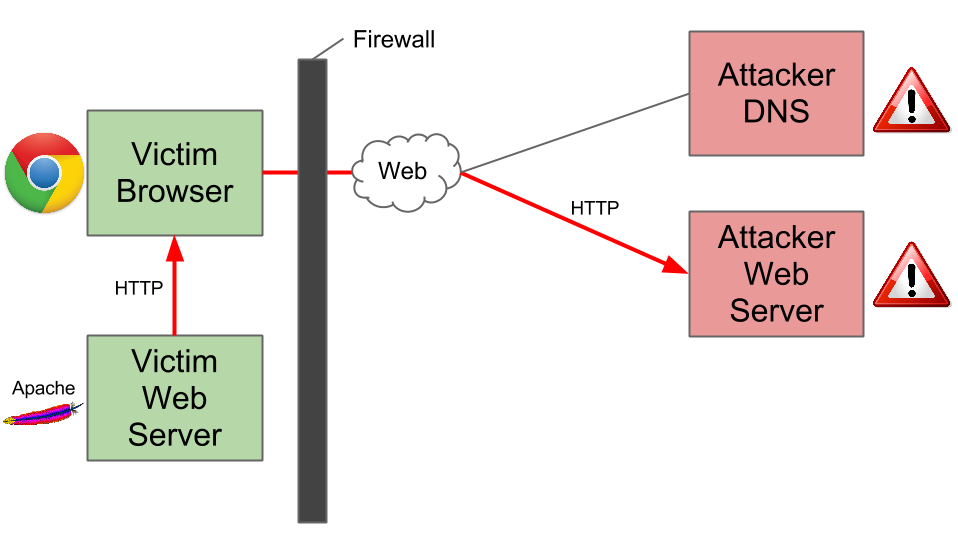
\includegraphics[width=0.8\columnwidth]{dnsrebind1.png}
\caption{\textbf{Traditional DNS Rebinding attack.} Once the victim's browser has established connection to both servers, it can relay data from the internal server back to the attacker's server.  The attacker can use this to gain access to private information stored on the victim's intranet.}
\label{fig:dnsrebind1}
\end{figure}


A common defense against the traditional attack is DNS pinning. With DNS pinning, the browser will cache the result of the DNS lookup for a period of time regardless of the response's TTL. This defense is not entirely effective though, as browser plug-ins generally maintain separate DNS entry databases. Such \emph{multi-pin} vulnerabilities are the result of each plug-in mapping to a different IP address, and then communicating with one another in order to execute the attack. However, many multi-pin vulnerabilities have been closed as well by the developers of the plug-ins. 

Our work focuses on executing a DNS rebinding attack by flooding the DNS cache used for DNS pinning on the victim's browser. We flood the cache with invalid entries in order to force the browser to do the vital second DNS lookup. In order to demonstate this exploit, we implement FireDrill, a tool that uses this vulnerability to initialize a fully interactive session between the attacker and the victim's web server.

The rest of the paper is organized as follows: Section 2 discusses related work on DNS rebinding. Section 3 introduces the cache flooding exploit and outlines our implementation of FireDrill. Section 4 evaluates this technique against alternative approaches. Section 5 discusses defenses and future work. Section 6 concludes.
